\documentclass[tikz]{standalone}
\usepackage{amsmath}
\usetikzlibrary{arrows}
\begin{document}
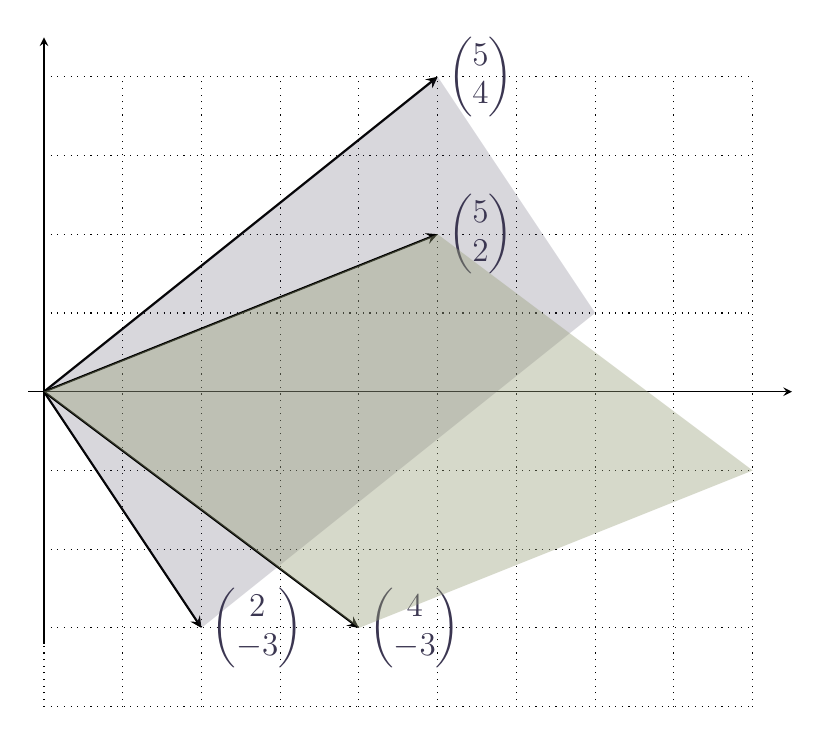
\begin{tikzpicture}[scale=1.0]

% ------------------------------------------------ lin_alg theme colors
\definecolor{la_white}{RGB}{233,235,223} %#E9EBDF
\definecolor{la_dark}{RGB}{59,54,81}     %#3B3651
\definecolor{la_gray}{RGB}{96,112,139}   %#60708B
\definecolor{la_tan}{RGB}{152,159,122}   %#989F7A

% axes
  \draw[thin,>=stealth,->]           (0,-3.2) -- (0,4.5);
  \draw[thin,>=stealth,->]           (-0.2,0) -- (9.5,0);

% grid lines
   \draw[step=1.0,black,thin,dotted,xshift=1cm,yshift=1cm] (-1,-5) grid (8,3);
    
\draw[thick,>=stealth,->,draw=black] (0,0) -- (5,4)   node[right, text=la_dark,  text width=5em] {\large $\mathbf{ \begin{pmatrix} 5 \\ 4 \end{pmatrix} }$} ;
\draw[thick,>=stealth,->,draw=black] (0,0) -- (2,-3)  node[right, text=la_dark,  text width=5em] {\large $\mathbf{ \begin{pmatrix} 2 \\ -3 \end{pmatrix} }$} ;
\fill[color=la_dark,fill=la_dark,fill opacity=0.2] (0,0) -- (5,4) -- (7,1) -- (2,-3) -- cycle;

\draw[thick,>=stealth,->,draw=black] (0,0) -- (5,2)   node[right, text=la_dark,  text width=5em] {\large $\mathbf{ \begin{pmatrix} 5 \\ 2 \end{pmatrix} }$} ;
\draw[thick,>=stealth,->,draw=black] (0,0) -- (4,-3)  node[right, text=la_dark,  text width=5em] {\large $\mathbf{ \begin{pmatrix} 4 \\ -3 \end{pmatrix} }$} ;
\fill[color=la_dark,fill=la_tan,fill opacity=0.4] (0,0) -- (5,2) -- (9,-1) -- (4,-3) -- cycle;

% starting vector blue, transformed vector red
%  \draw[thick,>=stealth,->,draw=black] (0,0) -- (5,1)  node[right, text=blue,  text width=5em] {\large $\mathbf{\begin{pmatrix} 5 \\ 1 \end{pmatrix}}$};
%  \draw[thick,>=stealth,->,dotted,draw=black] (5,1) -- (2,1);
%  \draw[thick,>=stealth,->,draw=black] (0,0) -- (1,3)  node[text=blue, label={[xshift=0.3cm, yshift=-0.1cm]\large $\color{blue}{\mathbf{\begin{pmatrix} 1 \\ 3 \end{pmatrix}}}$}] (x2) {};
%  \draw[thick,>=stealth,->,dotted,draw=black] (1,3) -- (6,3);

\end{tikzpicture}
\end{document}